\documentclass[12pt]{article}
\usepackage[utf8]{inputenc}
\usepackage{graphicx}
\usepackage{amsmath}
\usepackage{amssymb}
\usepackage{booktabs}
\usepackage{float}
\usepackage{geometry}
\usepackage{hyperref}

\geometry{a4paper, margin=1in}

\title{Three-Layer Neural Network Classifier Experiment Report}
\author{Long Zhuohan \\ Student ID: 24210980127}
\date{\today}

\begin{document}

\maketitle

\section{Project Links}
\begin{itemize}
    \item GitHub Repository: \url{https://github.com/NanshineLoong/3-layer-Neural-Network.git}
    \item Model Weights: \url{https://drive.google.com/file/d/16fqyr1Jc7LstVuPjikmTfwYNS53UcDph/view?usp=sharing}
\end{itemize}

\section{Experiment Purpose}
This experiment aims to build a three-layer neural network classifier from scratch and train it on the CIFAR-10 dataset for image classification. By manually implementing the backpropagation algorithm, we gain a deep understanding of how neural networks work and the training process.

\section{Experiment Environment}
\begin{itemize}
    \item Operating System: macOS
    \item Python Version: 3.8
    \item Main Dependencies: NumPy, Matplotlib, scikit-learn, tqdm
\end{itemize}

\section{Experiment Content}

\subsection{Dataset}
Using the CIFAR-10 dataset, which contains 60,000 32x32 color images in 10 classes:
\begin{itemize}
    \item Training Set: 50,000 images
    \item Test Set: 10,000 images
    \item Classes: airplane, automobile, bird, cat, deer, dog, frog, horse, ship, truck
\end{itemize}

\subsection{Model Architecture}
\begin{itemize}
    \item Input Layer: 3,072 neurons (32x32x3 image)
    \item Hidden Layer: 128 neurons
    \item Output Layer: 10 neurons (corresponding to 10 classes)
    \item Activation Functions: ReLU (hidden layer), Sigmoid (output layer)
    \item Loss Function: Cross-entropy loss
    \item Optimizer: SGD (Stochastic Gradient Descent)
    \item Regularization: L2 regularization
\end{itemize}

\subsection{Training Process}
\begin{itemize}
    \item Training Epochs: 100
    \item Batch Size: 64
    \item Initial Learning Rate: 0.01
    \item Learning Rate Decay: 5\% every 10 epochs
    \item L2 Regularization Strength: 0.01
\end{itemize}

\section{Experiment Results}

\subsection{Training Curves}
\begin{figure}[H]
    \centering
    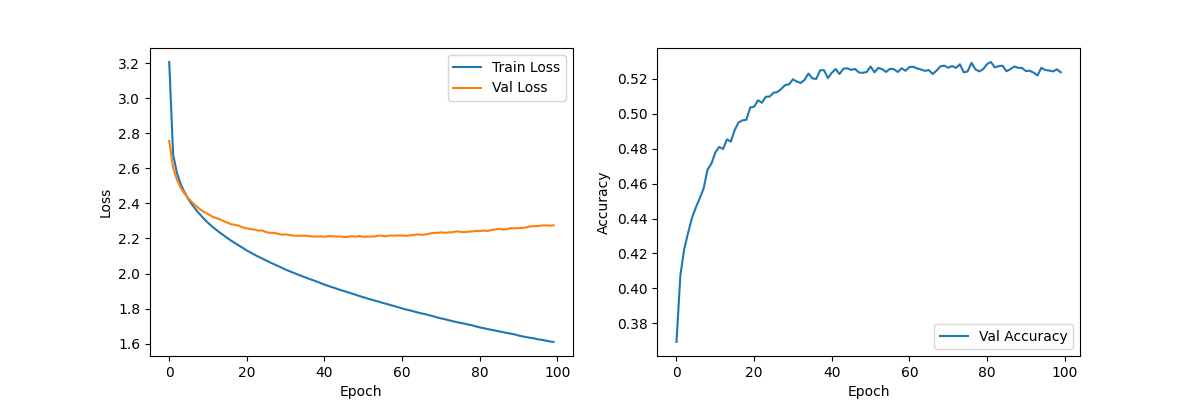
\includegraphics[width=0.8\textwidth]{results/training_curves.png}
    \caption{Training and validation loss curves, and validation accuracy curve}
    \label{fig:training_curves}
\end{figure}

\subsection{Model Weights Visualization}
\begin{figure}[H]
    \centering
    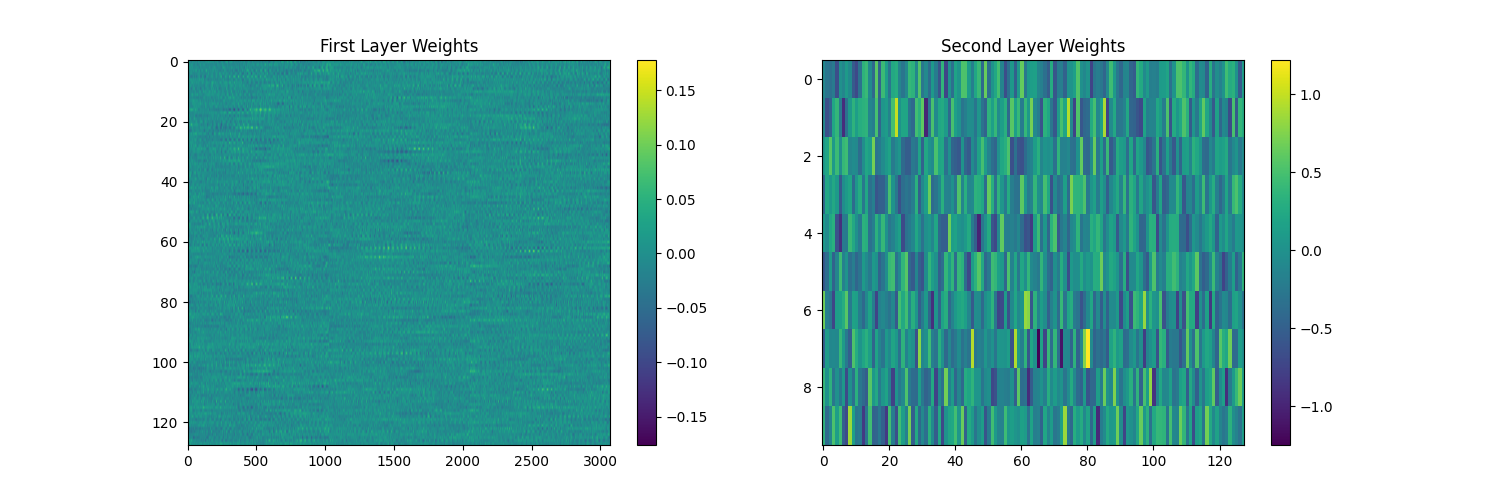
\includegraphics[width=0.8\textwidth]{results/weights_visualization.png}
    \caption{Model weights visualization}
    \label{fig:weights}
\end{figure}

\subsection{Class-wise Accuracy}
\begin{figure}[H]
    \centering
    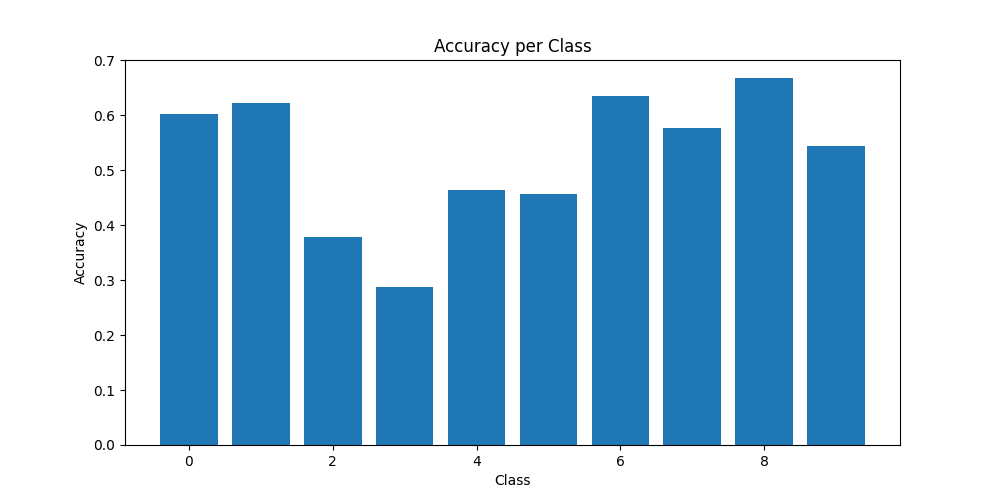
\includegraphics[width=0.8\textwidth]{results/class_accuracies.png}
    \caption{Test set accuracy for each class}
    \label{fig:class_acc}
\end{figure}

\subsection{Performance Metrics}
\begin{table}[H]
    \centering
    \begin{tabular}{lc}
        \toprule
        Metric & Value \\
        \midrule
        Final Training Loss & 1.6097 \\
        Final Validation Loss & 2.2755 \\
        Validation Accuracy & 52.37\% \\
        Test Accuracy & 52.35\% \\
        \bottomrule
    \end{tabular}
    \caption{Model performance metrics}
    \label{tab:metrics}
\end{table}

\subsection{Detailed Class-wise Accuracy}
\begin{table}[H]
    \centering
    \begin{tabular}{lc}
        \toprule
        Class & Accuracy \\
        \midrule
        Airplane & 66.70\% \\
        Automobile & 62.30\% \\
        Bird & 37.90\% \\
        Cat & 28.70\% \\
        Deer & 46.40\% \\
        Dog & 45.60\% \\
        Frog & 63.50\% \\
        Horse & 57.70\% \\
        Ship & 66.70\% \\
        Truck & 54.40\% \\
        \bottomrule
    \end{tabular}
    \caption{Test set accuracy for each class}
    \label{tab:class_acc}
\end{table}

\section{Experiment Analysis}

\subsection{Model Performance Analysis}
\begin{itemize}
    \item The model achieved 52.35\% accuracy on the test set, very close to the validation accuracy (52.37\%), indicating no overfitting
    \item There is significant variation in accuracy across classes, with the highest (airplane, ship: 66.70\%) and lowest (cat: 28.70\%) differing by about 38 percentage points
    \item Training loss decreased consistently from 3.2066 to 1.6097, indicating good learning progress
\end{itemize}

\subsection{Improvement Directions}
\begin{itemize}
    \item Replace fully connected network with Convolutional Neural Network (CNN) to better capture spatial features
    \item Increase network depth to improve model expressiveness
    \item Add data augmentation to enhance model generalization
    \item Use more sophisticated optimizers (e.g., Adam) instead of SGD
    \item Fine-tune learning rate and regularization parameters to find better hyperparameter combinations
\end{itemize}

\section{Experiment Summary}
Through this experiment, we successfully implemented a three-layer neural network classifier and trained it on the CIFAR-10 dataset. Although the model's accuracy is not very high, by manually implementing the backpropagation algorithm, we gained a deep understanding of how neural networks work. The results show that simple fully connected networks have certain limitations in handling image classification tasks, which provides direction for future improvements.

\end{document} 